\documentclass[12pt]{report}
\usepackage[utf8]{inputenc}
\usepackage[russian]{babel}
%\usepackage[14pt]{extsizes}
\usepackage{listings}
\usepackage{graphicx}
\usepackage{amsmath,amsfonts,amssymb,amsthm,mathtools} 
\usepackage{pgfplots}
\usepackage{filecontents}
\usepackage{float}
\usepackage{comment}
\usepackage{indentfirst}
\usepackage{eucal}
\usepackage{enumitem}
%s\documentclass[openany]{book}
\frenchspacing

\usepackage{indentfirst} % Красная строка

\usetikzlibrary{datavisualization}
\usetikzlibrary{datavisualization.formats.functions}

\usepackage{amsmath}


% Для листинга кода:
\lstset{ %
	language=c,                 % выбор языка для подсветки (здесь это С)
	basicstyle=\small\sffamily, % размер и начертание шрифта для подсветки кода
	numbers=left,               % где поставить нумерацию строк (слева\справа)
	numberstyle=\tiny,           % размер шрифта для номеров строк
	stepnumber=1,                   % размер шага между двумя номерами строк
	numbersep=5pt,                % как далеко отстоят номера строк от подсвечиваемого кода
	showspaces=false,            % показывать или нет пробелы специальными отступами
	showstringspaces=false,      % показывать или нет пробелы в строках
	showtabs=false,             % показывать или нет табуляцию в строках
	frame=single,              % рисовать рамку вокруг кода
	tabsize=2,                 % размер табуляции по умолчанию равен 2 пробелам
	captionpos=t,              % позиция заголовка вверху [t] или внизу [b] 
	breaklines=true,           % автоматически переносить строки (да\нет)
	breakatwhitespace=false, % переносить строки только если есть пробел
	escapeinside={\#*}{*)}   % если нужно добавить комментарии в коде
}


\usepackage[left=2cm,right=2cm, top=2cm,bottom=2cm,bindingoffset=0cm]{geometry}
% Для измененных титулов глав:
\usepackage{titlesec, blindtext, color} % подключаем нужные пакеты
\definecolor{gray75}{gray}{0.75} % определяем цвет
\newcommand{\hsp}{\hspace{20pt}} % длина линии в 20pt
% titleformat определяет стиль
\titleformat{\chapter}[hang]{\Huge\bfseries}{\thechapter\hsp\textcolor{gray75}{|}\hsp}{0pt}{\Huge\bfseries}


% plot
\usepackage{pgfplots}
\usepackage{filecontents}
\usetikzlibrary{datavisualization}
\usetikzlibrary{datavisualization.formats.functions}

\begin{document}
	%\def\chaptername{} % убирает "Глава"
	\thispagestyle{empty}
	\begin{titlepage}
		\noindent \begin{minipage}{0.15\textwidth}
			
\includegraphics[width=\linewidth]{img/b_logo}
		\end{minipage}
		\noindent\begin{minipage}{0.9\textwidth}\centering
			\textbf{Министерство науки и высшего образования Российской Федерации}\\
			\textbf{Федеральное государственное бюджетное образовательное учреждение высшего образования}\\
			\textbf{~~~«Московский государственный технический университет имени Н.Э.~Баумана}\\
			\textbf{(национальный исследовательский университет)»}\\
			\textbf{(МГТУ им. Н.Э.~Баумана)}
		\end{minipage}
		
		\noindent\rule{18cm}{3pt}
		\newline\newline
		\noindent ФАКУЛЬТЕТ $\underline{\text{«Информатика и системы управления»}}$ \newline\newline
		\noindent КАФЕДРА $\underline{\text{«Программное обеспечение ЭВМ и информационные технологии»}}$\newline\newline\newline\newline\newline
		
		\begin{center}
			\noindent\begin{minipage}{1.1\textwidth}\centering
				\Large\textbf{  Отчет по лабораторной работе №9}\newline
				\textbf{по дисциплине <<Компьютерные сети>>}\newline\newline\newline
			\end{minipage}
		\end{center}
		
		\noindent\textbf{Тема} $\underline{\text{
		Изучение технологии виртуальных локальный сетей (VLAN)}}$\newline\newline
		\noindent\textbf{Студент} $\underline{\text{Романов А.В.~~~~~~~~~~~}}$\newline\newline
		\noindent\textbf{Группа} $\underline{\text{ИУ7-73Б~~~~~~~~~~~~~~~~~~~}}$\newline\newline
		\noindent\textbf{Преподаватель} $\underline{\text{Рогозин Н. О.}}$\newline\newline\newline
		
		\begin{center}
			\vfill
			Москва~---~\the\year
			~г.
		\end{center}
	\end{titlepage}


\section*{Задание}

\textbf{Вариант №12.}\\

Необходимо:

\begin{enumerate}
	\item назначить адреса подсетей:
	\begin{itemize}
		\item подсеть 1: 192.168.x.0 /24
		\item подсеть 2: 192.168.x+1.0 /24
		\item подсеть 3: 192.168.x+2.0 /24
	\end{itemize}
	\item настроить поддержку трех виртуальных локальных сетей (VLan 10, 20, 30) на коммутаторе;
	\item настроить маршрутизацию между виртуальными локальными сетями на маршрутизаторе;
	\item выделить и озаглавить на схеме каждую виртуальную локальную сеть.
\end{enumerate}

\section*{Результаты работы}

\subsection*{Разделение на подсети}

В ходе выполнения работы были назначены адреса подсетей в соответствии с заданием.

\subsection*{Настройка поддержки виртуальных сетей}

На рисунках \ref{fig:1} - \ref{fig:2} представлены команды, которые были выполнены на коммутаторе для его настройки.

\begin{figure}[H]
	\begin{center}
		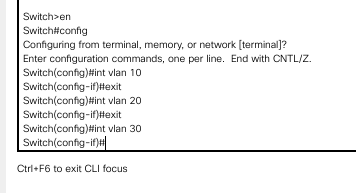
\includegraphics[scale=0.7]{img/1.png}
	\end{center}
	\caption{Настройка коммутатора, первая часть}
	\label{fig:1}
\end{figure}

\begin{figure}[H]
	\begin{center}
		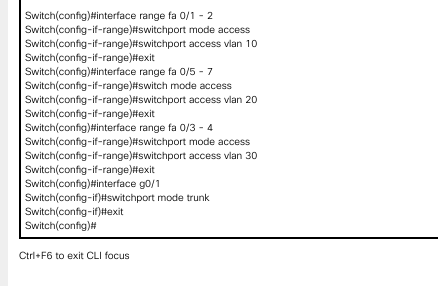
\includegraphics[scale=0.7]{img/2.png}
	\end{center}
	\caption{Настройка коммутатора, вторая часть}
	\label{fig:2}
\end{figure}

На рисунке \ref{fig:3} представлен список виртуальных сетей.

\begin{figure}[H]
	\begin{center}
		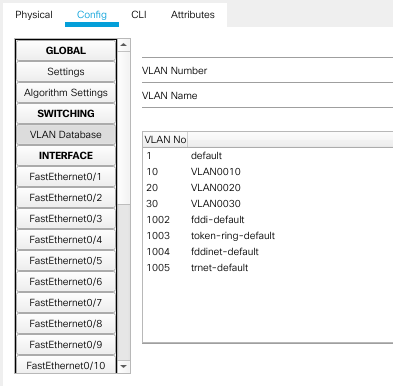
\includegraphics[scale=0.7]{img/3.png}
	\end{center}
	\caption{Список виртуальных сетей на коммутаторе}
	\label{fig:3}
\end{figure}

На рисунке \ref{fig:4} представлен список физических интерфейсов коммутатора.

\begin{figure}[H]
	\begin{center}
		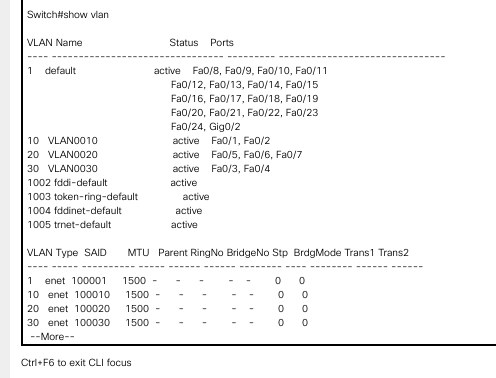
\includegraphics[scale=0.7]{img/4.png}
	\end{center}
	\caption{Список физических интерфейсов коммутатора}
	\label{fig:4}
\end{figure}

\subsection*{Настройка маршрутизации между виртуальными сетями}

На рисунке \ref{fig:5} представлены команды, которые были выполнены для настройки маршрутизации между виртуальными локальными сетями на маршрутизаторе.

\begin{figure}[H]
	\begin{center}
		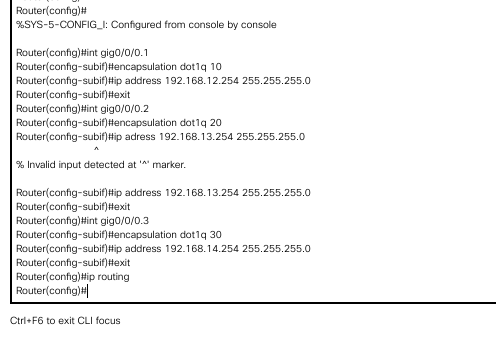
\includegraphics[scale=0.7]{img/5.png}
	\end{center}
	\caption{Выделенные виртуальные сети}
	\label{fig:5}
\end{figure}

Были созданы три подинтерфейса (рисунок \ref{fig:6}).

\begin{figure}[H]
	\begin{center}
		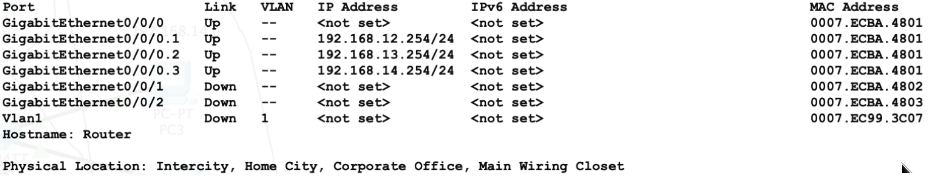
\includegraphics[scale=0.7]{img/6.png}
	\end{center}
	\caption{Список интерфейсов маршрутизатора}
	\label{fig:6}
\end{figure}

\subsection*{Выделение виртуальных сетей}

На рисунке \ref{fig:7} представлены выделенные в ходе работы виртуальные локальные сети.

\begin{figure}[H]
	\begin{center}
		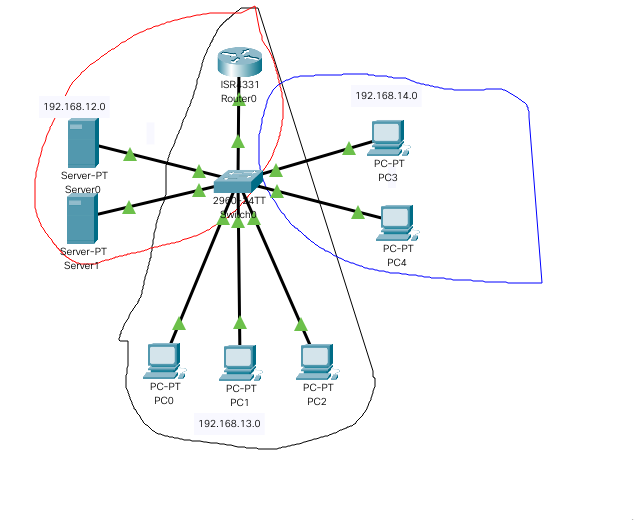
\includegraphics[scale=0.7]{img/7.png}
	\end{center}
	\caption{Выделенные виртуальные сети}
	\label{fig:7}
\end{figure}

На рисунке \ref{fig:8} представлен результат проверки соединения.

\begin{figure}[H]
	\begin{center}
		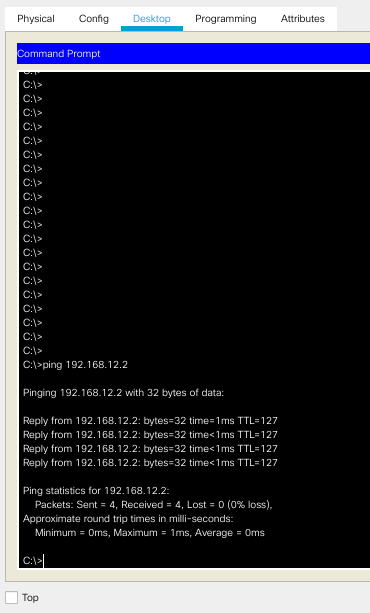
\includegraphics[scale=0.8]{img/8.png}
	\end{center}
	\caption{Проверка соединения с помощью команды \texttt{ping}}
	\label{fig:8}
\end{figure}

\bibliographystyle{utf8gost705u}
\bibliography{51-biblio}
	
\end{document}
